% HMC Math dept HW template example
% v0.04 by Eric J. Malm, 10 Mar 2005
\documentclass[12pt,letterpaper,boxed,cm]{hmcpset}

% set 1-inch margins in the document
\usepackage[margin=1in]{geometry}
\usepackage{mathtools}
\usepackage{mathrsfs}
% include this if you want to import graphics files with /includegraphics
\usepackage{graphicx}
\usepackage{cases}
\usepackage{hyperref}
\usepackage{siunitx}
\usepackage{tikz}
\usepackage{cases}
\usetikzlibrary{arrows}

% info for header block in upper right hand corner
\name{Name: ~~~~~~~~~~~~~~~~~~~~~~~~~~~}
\class{Physics 51}
\assignment{Homework \#12}
\duedate{October 13, 2016}

\newcommand{\ev}[2]{\Big|_{#1}^{#2}}
\newcommand{\evv}[2]{\Big|_{#1}^{#2}}
\newcommand{\set}[1]{\left\{#1\right\}}
\newcommand{\s}[1]{\sqrt{#1}}
\newcommand{\f}[2]{\frac{#1}{#2}}
\newcommand{\p}[2]{\frac{\partial #1}{\partial #2}}
\providecommand{\t}[1]{\text{#1}}
\providecommand{\span}[1]{\text{span}\left(#1\right)}
\providecommand{\set}[1]{\left\{#1\right\}}
\providecommand{\l}[0]{\left}
\providecommand{\r}[0]{\right}
\newcommand{\m}[1]{\begin{matrix}#1\end{matrix}}
\newcommand{\bm}[1]{\begin{bmatrix}#1\end{bmatrix}}
\renewcommand{\bf}[1]{\mathbf{#1}}
\newcommand{\pn}[1]{\left( #1 \right)}
\newcommand{\abs}[1]{\left| #1 \right|}
\newcommand{\bk}[1]{\left[ #1 \right]}
\newcommand{\cis}[1]{\pn{\cos\pn{#1} + i\sin\pn{#1}}}
\newcommand{\cisi}[1]{\pn{\cos\pn{#1} - i\sin\pn{#1}}}
\renewcommand{\Im}[1]{\text{Im}\pn{#1}}
\renewcommand{\Re}[1]{\text{Re}\pn{#1}}
\renewcommand{\k}[0]{\f{1}{4\pi\epsilon_0}}
\renewcommand{\part}[1]{\vspace{1em}\noindent(#1)}

\makeatletter
\renewcommand*\env@matrix[1][*\c@MaxMatrixCols c]{%
  \hskip -\arraycolsep
  \let\@ifnextchar\new@ifnextchar
  \array{#1}}
\makeatother
\begin{document}
\problemlist{32-P10, SUP21, SUP22}

\begin{problem}[32-P10]
In Bohr's theory of the hydrogen atom, the electron can be thought of as moving in a circular orbit of radius $r$ about the proton. Suppose that such an atom is placed in a magnetic field, with the plane of the orbit at right angles to $\vec{\mathbf{B}}$. 
\begin{enumerate}
	\item[(a)] If the electron is circulating clockwise, as viewed by an observer sighting along $\vec{\mathbf{B}}$, will the angular frequency increase or decrease?
	\item[(b)] What if the electron is circulating counterclockwise? Assume that the orbit radius does not change [Hint: The centripetal force is now partially electric ($\vec{\mathbf{F}}_E$) and partially magnetic ($\vec{\mathbf{F}}_B$) in origin.]
	\item[(c)] Show that the change in frequency of revolution caused by the magnetic field is given approximately by
\[
	\Delta f = \pm \f{Be}{4\pi m}.
\]
	Such frequency shifts were observed by Zeeman in 1896. (Hint: Calculate the frequency of revolution without the magnetic field and also with it. Subtract, bearing in mind that because the effect of the magnetic field is very small, some--but not all--terms containing $B$ can be set equal to zero with little error.)
\end{enumerate}
\end{problem}
\begin{solution}
\end{solution}
\newpage

\begin{problem}[SUP21]
Consider a rectangular wire loop of sides $a$ and $b$ carrying a current $i$. The current-carrying loop is immersed in a uniform magnetic field $B$. The loop is oriented so that side $b$ is perpendicular to the magnetic field and side $a$ is tilted at some angle, so that the angle between the magnetic field and $\hat{n}$ the normal to the loop is $\theta$. Show that the torque on the current loop is given by:
\[
	\vec{\tau} = \vec{\mu} \times \vec{B}
\]
where $\vec{\mu} = iab~\hat{n}$ is called the \textit{magnetic dipole moment} of the loop.
\end{problem}
\begin{solution}
\end{solution}
\newpage

\begin{problem}[SUP22]
A current $i$ flows in a thin semi-infinite wire. At the cut-off end of the wire, assume the flowing charge builds up in a point-like accumulation. Determine the magnetic field at a perpendicular distance $R$ from the wire end using the following three approaches, verifying that they give the same results:
\begin{enumerate}
	\item[(a)] Use Ampère's Law with the hemispherical surface $S_1$ (see diagram) that intersects the wire.
	\item[(b)] Use Ampère's Law with the hemispherical surface $S_2$ that \textit{does not} intersect the wire.
	\item[(c)] Use the Biot-Savart Law.
\end{enumerate}
\begin{center}
	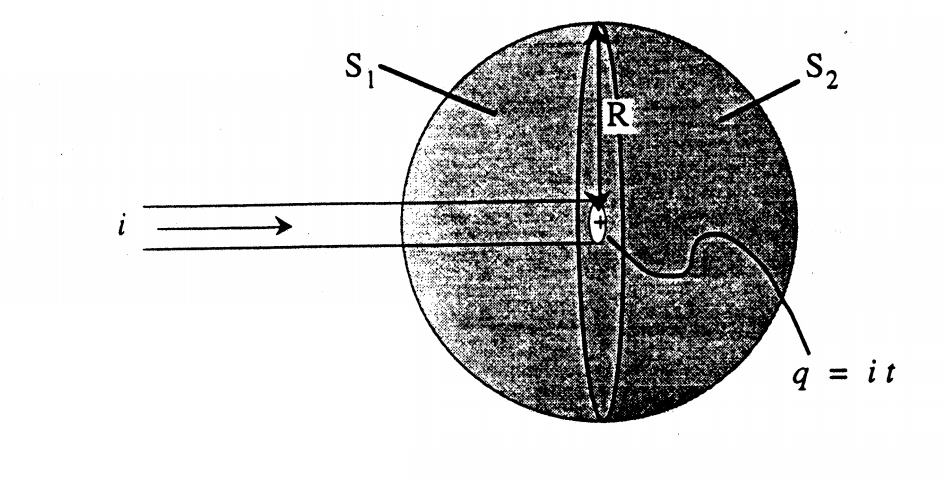
\includegraphics[scale=0.5]{pic01.png}	
\end{center}
\end{problem}
\begin{solution}
\end{solution}

\end{document}